\documentclass[]{article}
\usepackage{lmodern}
\usepackage{amssymb,amsmath}
\usepackage{ifxetex,ifluatex}
\usepackage{fixltx2e} % provides \textsubscript
\ifnum 0\ifxetex 1\fi\ifluatex 1\fi=0 % if pdftex
  \usepackage[T1]{fontenc}
  \usepackage[utf8]{inputenc}
\else % if luatex or xelatex
  \ifxetex
    \usepackage{mathspec}
    \usepackage{xltxtra,xunicode}
  \else
    \usepackage{fontspec}
  \fi
  \defaultfontfeatures{Mapping=tex-text,Scale=MatchLowercase}
  \newcommand{\euro}{€}
\fi
% use upquote if available, for straight quotes in verbatim environments
\IfFileExists{upquote.sty}{\usepackage{upquote}}{}
% use microtype if available
\IfFileExists{microtype.sty}{%
\usepackage{microtype}
\UseMicrotypeSet[protrusion]{basicmath} % disable protrusion for tt fonts
}{}
\usepackage[margin=1in]{geometry}
\usepackage{graphicx}
\makeatletter
\def\maxwidth{\ifdim\Gin@nat@width>\linewidth\linewidth\else\Gin@nat@width\fi}
\def\maxheight{\ifdim\Gin@nat@height>\textheight\textheight\else\Gin@nat@height\fi}
\makeatother
% Scale images if necessary, so that they will not overflow the page
% margins by default, and it is still possible to overwrite the defaults
% using explicit options in \includegraphics[width, height, ...]{}
\setkeys{Gin}{width=\maxwidth,height=\maxheight,keepaspectratio}
\ifxetex
  \usepackage[setpagesize=false, % page size defined by xetex
              unicode=false, % unicode breaks when used with xetex
              xetex]{hyperref}
\else
  \usepackage[unicode=true]{hyperref}
\fi
\hypersetup{breaklinks=true,
            bookmarks=true,
            pdfauthor={Benjamin Weigel},
            pdftitle={WEB346 - flavones - peculiar products},
            colorlinks=true,
            citecolor=blue,
            urlcolor=blue,
            linkcolor=magenta,
            pdfborder={0 0 0}}
\urlstyle{same}  % don't use monospace font for urls
\setlength{\parindent}{0pt}
\setlength{\parskip}{6pt plus 2pt minus 1pt}
\setlength{\emergencystretch}{3em}  % prevent overfull lines
\setcounter{secnumdepth}{0}

%%% Use protect on footnotes to avoid problems with footnotes in titles
\let\rmarkdownfootnote\footnote%
\def\footnote{\protect\rmarkdownfootnote}

%%% Change title format to be more compact
\usepackage{titling}

% Create subtitle command for use in maketitle
\newcommand{\subtitle}[1]{
  \posttitle{
    \begin{center}\large#1\end{center}
    }
}

\setlength{\droptitle}{-2em}
  \title{WEB346 - flavones - peculiar products}
  \pretitle{\vspace{\droptitle}\centering\huge}
  \posttitle{\par}
  \author{Benjamin Weigel}
  \preauthor{\centering\large\emph}
  \postauthor{\par}
  \predate{\centering\large\emph}
  \postdate{\par}
  \date{28.10.2015}



\begin{document}

\maketitle


\section{Flavones}\label{flavones}

Chromatograms that are available are highly biased (only at high pH with
Mg and wt, other conditions are highly underrepresented.). Chromatograms
(high pH, Mg, wt) show two products. One is the original 3' or 4'
methylated substrate (rt 14.55 min). The other elutes earlier than the
substrate, at 12.59, 12.69 and 12.78 min when apigenin, chrysoeriol or
diosmetin were substrates respectively. The fraction of this product to
the `true' product is in favour of the true product when a free
3'-hydroxyl (diosmetin) can be methylated. Otherwise it is shifted in
favor of the `false' product (apigenin, chrysoeriol).

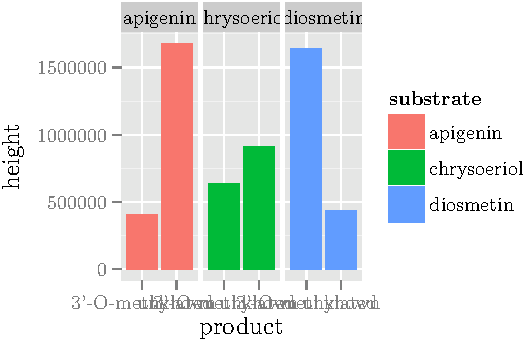
\includegraphics{flavones_products_files/figure-latex/unnamed-chunk-1-1.pdf}
\includegraphics{flavones_products_files/figure-latex/unnamed-chunk-1-2.pdf}
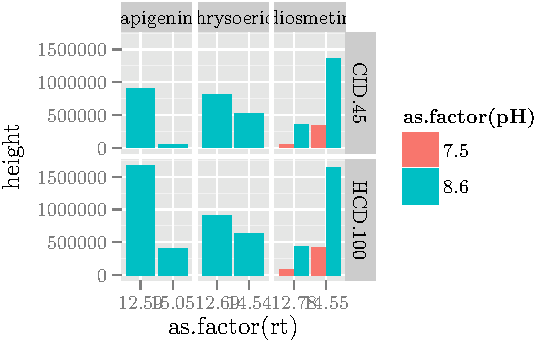
\includegraphics{flavones_products_files/figure-latex/unnamed-chunk-1-3.pdf}

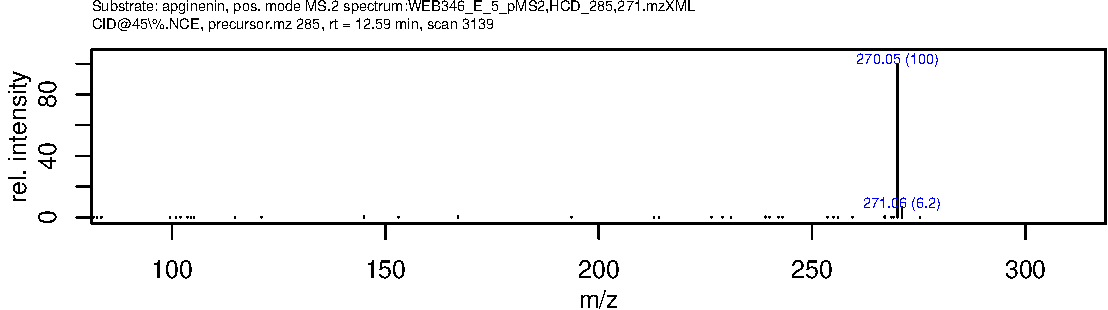
\includegraphics{flavones_products_files/figure-latex/tikz_plot-1.pdf}
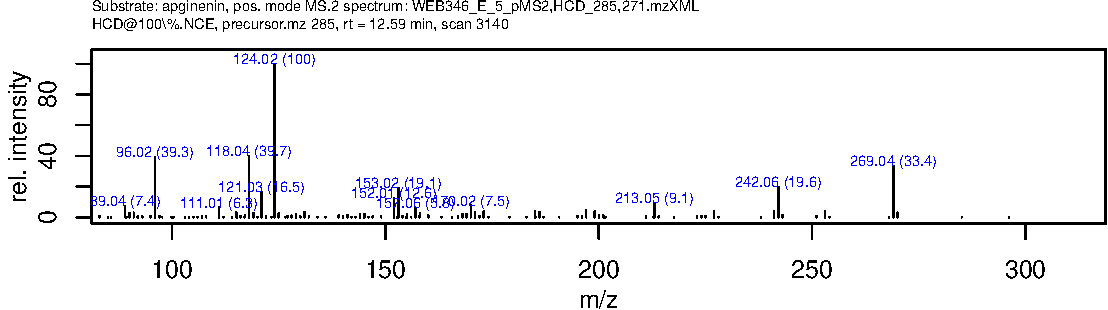
\includegraphics{flavones_products_files/figure-latex/tikz_plot-2.pdf}
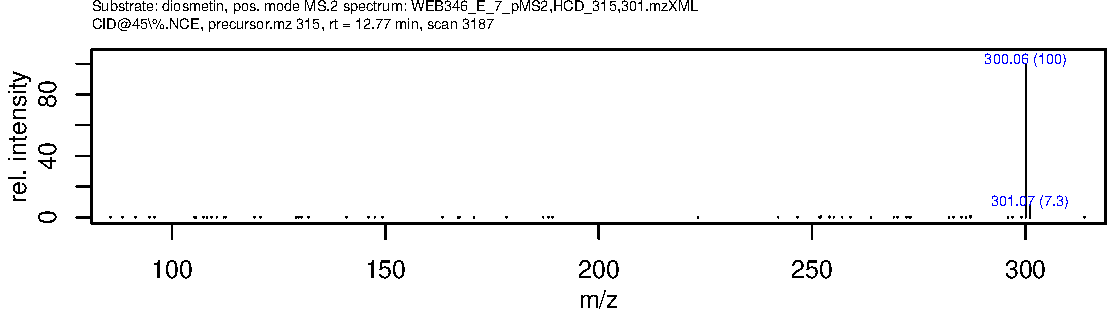
\includegraphics{flavones_products_files/figure-latex/tikz_plot-3.pdf}
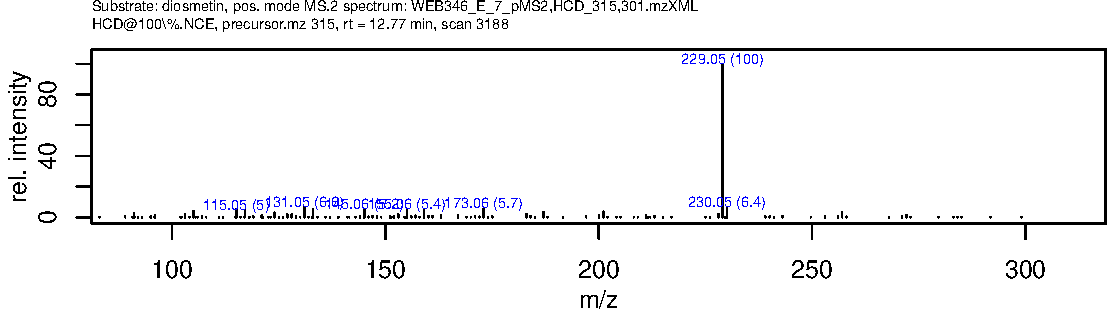
\includegraphics{flavones_products_files/figure-latex/tikz_plot-4.pdf}
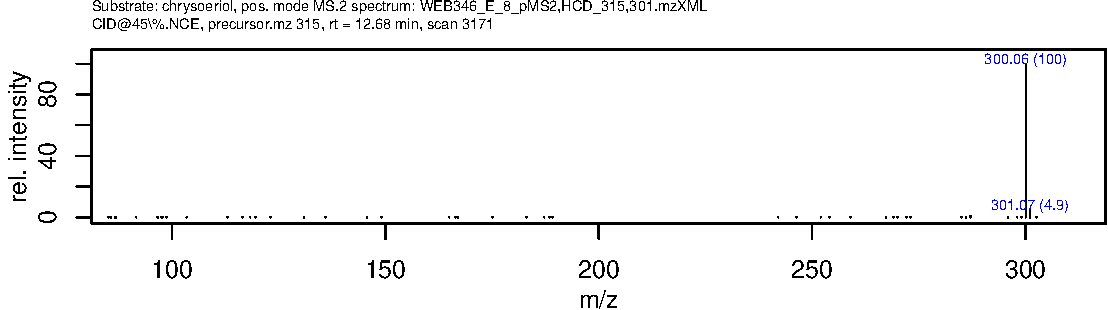
\includegraphics{flavones_products_files/figure-latex/tikz_plot-5.pdf}
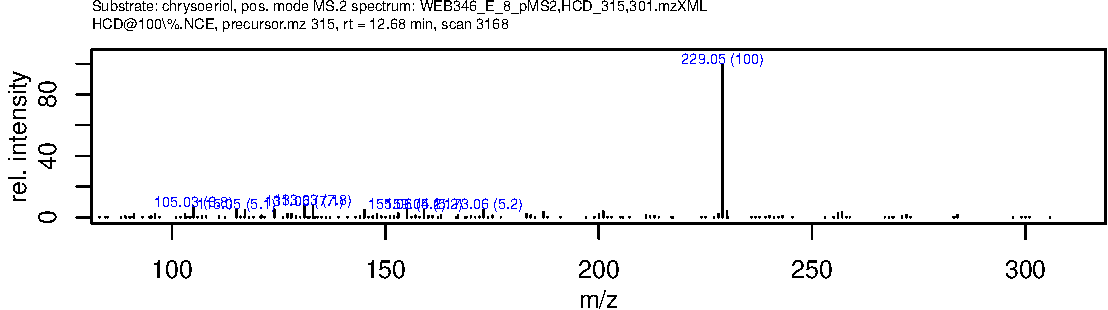
\includegraphics{flavones_products_files/figure-latex/tikz_plot-6.pdf}

\section{Flavonoles}\label{flavonoles}

\subsection{Kaempferol}\label{kaempferol}

some contaminations in substarte stock (rt 13.26, 15.22)

WEB346\_E\_15\_pMS2\_287,301.mzXML:

\begin{itemize}
\itemsep1pt\parskip0pt\parsep0pt
\item
  `product' peaks as 12.97 min and 14.1 min
\item
  14.1 min \textgreater{} CID does not produce fragments (just m/z 286)
  \textgreater{} no idea what \textgreater{} does not match any
  references
\item
  HCD spectrum shows characteristic 121, 136, 184, 213, 229, 258 and
  285/286
\item
  peak at 12.97 min
\item
  cid spectrum almost looks the same as peak 14.1 min
\item
  hcd spectrum also look s the same
\end{itemize}

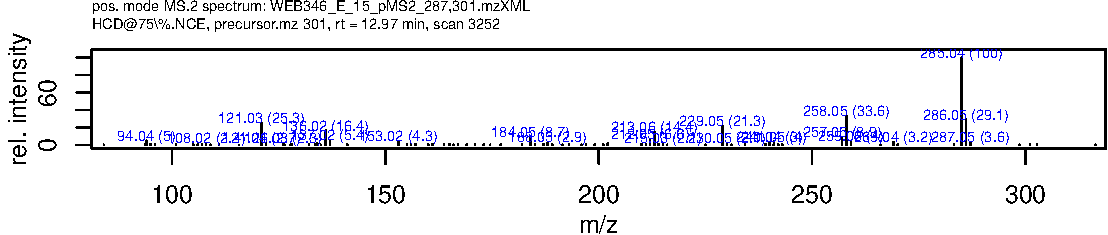
\includegraphics{flavones_products_files/figure-latex/kaempferol-1.pdf}
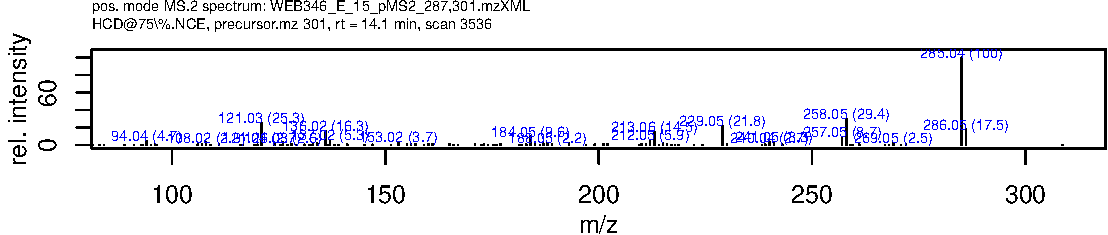
\includegraphics{flavones_products_files/figure-latex/kaempferol-2.pdf}

WEB346\_F\_15\_pMS2\_287,301.mzXML:

\begin{itemize}
\itemsep1pt\parskip0pt\parsep0pt
\item
  some peak at 14.11 min (same as WEB346\_E\_15\_pMS2\_287,301.mzXML)
  \textgreater{} does not match any reference spectra \textgreater{} no
  idea what
\end{itemize}

\subsection{Quercetin}\label{quercetin}

\textbf{product contamination in substrate stock!} (1.7e7 vs 4e5,
substrate vs product in cid)

WEB346\_B\_16\_pMS2\_303,317,331.mzXML:

\begin{itemize}
\itemsep1pt\parskip0pt\parsep0pt
\item
  mono-methyl product isorhamnetin at 13.98 min (fits the reference
  spectrum) (2e6 vs 1e7)
\item
  di-methyl product at 14.17 min (M+H 331) (m/z 153 and CO losses
  observed in HCD, only {[}M+H-CH3{]}+ in CID)
\item
  other (very small) peaks disregarded
\end{itemize}

WEB346\_E\_16\_pMS2\_303,317,331.mzXML:

\begin{itemize}
\itemsep1pt\parskip0pt\parsep0pt
\item
  only mono-methyl product observed in chromatogram (1.4e5 vs 5e5)
\item
  peak at 12.04 min (when precursor ion 317)
\item
  other peculiar peaks in chromatograms
\end{itemize}

WEB346\_F\_16\_pMS2\_303,317,331.mzXML:

\begin{itemize}
\itemsep1pt\parskip0pt\parsep0pt
\item
  mono-methyl product at 13.98 min (spectrum fits isorhamnetin) (2e5 vs
  8e6)
\item
  dimethyl product observed at 14.17 min \textgreater{} same as for
  WEB346\_B\_16\_pMS2\_303,317,331.mzXML
\end{itemize}

\end{document}
